% !TEX root = main.tex

\subsection{有信息搜索}
在无信息搜索中,我们从不估计边界集中最有期望(promising)获得最优解的结点,而是无区别地选择当前边界集中第一个结点。
然而事实上,针对不同问题我们是有对结点的先验知识(apriori knowledge)的,即从当前结点到目标结点的开销有多大。
而这就是有信息搜索(informed),或者称为启发式搜索(heuristics)。

关键在于领域特定启发式函数$h(n)$的设计,它估计了从结点$n$到目标结点的开销(cost)。
注意满足目标状态的结点$h(n)=0$。

\subsubsection{贪心最优搜索(Greedy Best-First Search)}
直接使用$h(n)$对边界集进行排序,但这会导致贪心地选择\textbf{看上去}离目标结点开销最小的路径。

如果存在环路,贪心最优搜索是不完备的,会陷入死循环。

\subsubsection{A$^\star$搜索}
综合考虑当前已走的开销和未来估计的开销。
定义一个估值函数
\[f(n)=g(n)+h(n)\]
其中$g(n)$为路径到节点$n$的代价,$h(n)$为从$n$到目标节点的代价,采用$f(n)$对边界集内的节点进行排序。

$f(n)$需要满足下列两个性质。
\begin{definition}[可采纳的(admissibility)]
假设所有代价$c(n1\to n2)\geq\eps>0$,令$h^\star(n)$为从$n$到目标节点$\infty$的最优解\footnote{如果没有路径则$h^\star(n)=\infty$},若
\[\forall n:\;h(n)\leq h^\star(n)\]
则称$h(n)$是可采纳的。
即一个可采纳的启发式函数总是\textbf{低估}了当前结点到目标结点的真实开销(这样才能保证最优解不被排除)。
\end{definition}
\begin{definition}[一致性(consistency)/单调性(monotonicity)]
若对于所有的结点$n_1$和$n_2$,$h(n)$满足(三角不等式)
\[h(n_1)\leq c(n_1\to n_2)_h(n_2)\]
则称$h(n)$是单调的。
\end{definition}

\begin{theorem}
一致性蕴含可采纳性
\end{theorem}
\begin{analysis}
分类讨论
\begin{itemize}
	\item 当结点$n$没有到目标结点的路径,则$h(n)\leq h^\star(n)=\infty$恒成立
	\item 令$n=n_1\to n_2\to\cdots\to n_k$为从结点$n$到目标结点的最优路径,则可以用数学归纳法证明$\forall i:\;h(n_i)\leq h^\star(n_i)$,如下从后往前推
	\[h(n_{i})\leq c(n_i\to n_{i+1})+h(n_{i+1})\leq c(n_i\to n_{i+1}) + h^\star(n_{i+1})=h^(n_i)\]
\end{itemize}
\end{analysis}

\begin{theorem}
可采纳性蕴含最优性
\end{theorem}
\begin{analysis}
假设最优解有开销$C^\star$,则任何最优解一定会在开销大于$C^\star$的路径之前被展开。
因此在最优解展开之前的路径一定有开销$\leq C^\star$,最终我们一定会检测到最优解,而且次优解不会在最优解之前被检测。
\end{analysis}

做环检测可能导致找不到最优解

但如果满足单调性,有以下几个性质
\begin{proposition}
路径上的$f$一定是非递减的
\end{proposition}
\begin{analysis}
\[\begin{aligned}
f(n)&=g(n)+h(n)\\
&\leq g(n)+c(n\to n')+h(n')\\
&= g(n')+h(n')\\
&= f(n')
\end{aligned}\]
\end{analysis}

\begin{proposition}
如果$n_2$在$n_1$之后被扩展,则$f(n_1)\leq f(n_2)$
\end{proposition}
\begin{analysis}
$n_2$在边界上
$n_1$
\end{analysis}
\begin{proposition}
当$n$在任何小于$f$值得路径之前被展开
\end{proposition}
\begin{analysis}
\end{analysis}
\begin{proposition}
$A^\star$算法第一次展开某个状态时,它已经找到了到达那个状态的最小开销路径。
\end{proposition}
\begin{analysis}
\end{analysis}

若满足单调性,则进行环检测不会破坏最优性

\subsubsection{迭代加深$A^\star$(IDA)算法}
$A^\star$算法有和BFS或UCS同样的空间复杂性问题,而迭代加深$A^\star$算法同样解决空间复杂度的问题

\subsubsection{构造启发式函数}
常常需要考虑一个更加简单的问题,然后让$h(n)$为到达一个简单问题解的开销

\begin{example}
现有积木若干,积木可以放在桌子上,也可以放在另一块积木上面。
有两种操作:
\begin{enumerate}
	\item \verb'move(x,y)':把积木x放到积木y上面,前提是积木x和积木y上面都没有其他积木
	\item \verb'moveToTable(x)':把积木x放到桌子上,前提是积木x上面无其他积木,且积木x不在桌子上
\end{enumerate}
设计一个可采纳的启发式函数$h(n)$
\end{example}
\begin{analysis}
$h(n)=h_1(n)+h_2(n)$
\end{analysis}

\subsection{博弈树搜索}
博弈的一些前提
\begin{itemize}
	\item 两个博弈玩家
	\item 离散值:游戏和决策都可以映射到离散空间
	\item 有限的:只有有限的状态和可能的决策
	\item 零和博弈:完全竞争,即如果一个玩家胜利,则另外一个失去同样数量的收益
	\item 确定性的:没有牵涉到概率性事件,如色子、抛硬币等
	\item 完美信息博弈:状态的所有方面都可以被完全观察,即没有隐藏的卡牌
\end{itemize}

剪刀石头布是简单的一次性(one-shot)博弈
\begin{itemize}
	\item 一次移动
	\item 在博弈论中称为策略或范式博弈(strategic/normal form)
\end{itemize}

但很多游戏是牵涉到多步操作的
\begin{itemize}
	\item 轮回(turn-taking)游戏,如棋类
	\item 在博弈论中称为扩展形式博弈(extensive form)
\end{itemize}

两个玩家$A$(最大化己方收益)和$B$(最小化对方收益)
\begin{itemize}
	\item 状态集合$\mathcal{S}$
	\item 初始状态$I\in\mathcal{S}$
	\item 终止位置$T\subset\mathcal{S}$
	\item 后继:下一可能状态的集合
	\item 效益(utility)/收益(payoff)函数$V:T\mapsto\rr$,表明终止状态对$A$玩家有多好,对$B$玩家有多坏(都站在$A$角度给出)
\end{itemize}

minimax算法:自己选max,对方选min
\begin{itemize}
	\item 构建整棵博弈树,然后将终止/叶子结点标上收益
	\item 回溯整棵树,然后将每个结点都标记上收益
\[U(n)=
\begin{cases}
\min\{U(c):\;c \text{ is a child of } n\} & n \text{ is a Min node}\\
\max\{U(c):\;c \text{ is a child of } n\} & n \text{ is a Max node}
\end{cases}\]
\end{itemize}
\begin{figure}[H]
\centering
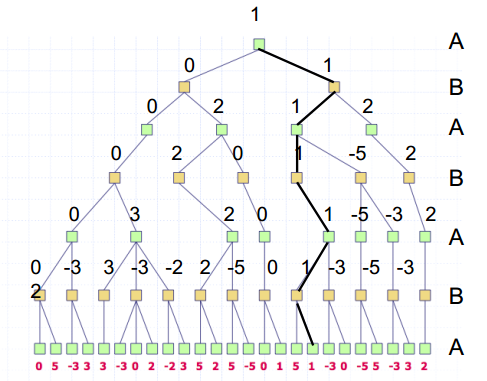
\includegraphics[width=0.6\linewidth]{fig/game-tree.png}
\end{figure}

用DFS可以遍历整棵树,同时保持线性的空间复杂度,每次回溯时更新结点为min/max即可

$\alpha$-$\beta$剪枝
\begin{itemize}
	\item 只要当前Max结点的值$\geq$祖先某一Min结点的值,就可以在该Max结点上做$\alpha$剪枝
	\item 只要当前Min结点的值$\leq$祖先某一Max结点的值,就可以在该Min结点上做$\alpha$剪枝
\end{itemize}
\begin{algorithm}
\caption{Alpha-Beta Pruning}
\begin{algorithmic}[1]
\Procedure{AlphaBeta}{n,Player,alpha,beta}
\If{n is TERMINAL}
\State \Return V(n)\Comment{Return terminal states utility}
\EndIf
\State ChildList = n.Successors(Player)
\If{Player == MAX}
\For{c in ChildList}
\State alpha = max(alpha, AlphaBeta(c,MIN,alpha,beta))
\If{beta <= alpha}
\State break
\EndIf
\EndFor
\State \Return alpha
\Else\Comment{Player == MIN}
\For{c in ChildList}
\State beta = min(beta, AlphaBeta(c,MAX,alpha,beta))
\If{beta <= alpha}
\State break
\EndIf
\EndFor
\State \Return beta
\EndIf
\EndProcedure\Comment{Initial call: AlphaBeta(START-NODE,Player,$-\infty$,$+\infty$)}
\end{algorithmic}
\end{algorithm}
可以证明,如果原始情况需要访问$O(b^D)$个结点,则经过$\alpha$-$\beta$剪枝后只需访问$O(b^{D/2})$个结点。

但在现实生活的游戏中,即使采用了$\alpha$-$\beta$剪枝,博弈树也太过庞大。
如棋类的分支因子大致是35,深度为10的树已经到$2.7\times 10^{14}$个结点。
因此不能将整棵博弈树展开,需要采用一些启发式方式进行估计。

评价函数(evaluation)的一些需求:
\begin{itemize}
	\item 对于终止状态,评价函数的序应与真实的收益函数相同
	\item 对于非终止状态,评价函数则应该与真实的胜率相关联
	\item 计算时间不能花太长
	\item 通常取多个特征,然后进行加权求和(先验知识)
\end{itemize}

在线(online)/实时(real-time)搜索
\begin{itemize}
	\item 没有办法展开全部的边界集,因此限制展开的大小(在没找到去目标的真实路径就做出决定/直接选一条路就开始走)
	\item 在这种情况下,评价函数不仅仅引导搜索,更是提交真实的动作
	\item 虽然找不到最优解,但是求解时间大大缩减
\end{itemize}